\scanpage{76}
\mspage{75}

part, \inserted{\handwritten{\uline{une fois choisi} \uline{une clôture} $\overline{\mathbb{F}}_p$,}}\handwritten{\begin{tikzpicture}[baseline=0cm,x=1cm,y=1cm]\draw[thin] (0,-.4)--(0,.15)..controls (0,.22) and (.2,.21)..(.45,.21)--(4.5,.25)..controls (5.2,.18) and (5.4,.2)..(5.5,.55);\end{tikzpicture}} la gerbe $\handwritten{\underline{\pi}}_p(\underline{F}_p)$, grâce àu\deleted{son} foncteur \unsure{\rlap{e}f|f}\unsure{\rlap{v}i|v|i|ï}bre évident ``fibre en $\handwritten{\bar{\underline{F}}}_p$ '' sur la catégorie des $\underline{Q}_p$-faisceaux constructibles sur $\underline{F}_p$, s'identifie à la \deleted{catégorie}\inserted{gerbe triviale définie\deleted{\unsure{et}} par .l'}enveloppe $\underline{Q}_p$-alg\unsure{e|é}briqueque du groupe profini $\handwritten{\pi}_1(\underline{F}_p)=\handwritten{\bar{\underline{Z}}}\deleted{r}$, \deleted{lequel, comme on le constate aisément, est le}

Un \inserted{$\underline{Q}_p$-}\handwritten{\begin{tikzpicture}[baseline=0cm,x=1cm,y=1cm]\draw[thin] (0,-.3)..controls (-.05,-.05) and (.55,.05)..(.7,.5);\end{tikzpicture}}faisceau constructible sur $\underline{F}_p$ s'identifie à un vectoriel de dimension finie $E$ sur $\underline{Q}_p$, muni d'un automorphisme $F_E$ tel que l'\deleted{hom} opération $n\handwritten{\mapsto}F_E^n$ de $\underline{Z}$ sur $E$ se prolonge par continuité en une opération de \deleted{\unsure{$\hat{\underline{Z}}_r$|$\hat{\underline{Z}}r$}} $\handwritten{\hat{\underline{Z}}}$ \margin{\handwritten{$Z$}}. Identifiant \inserted{\handwritten{(par un foncteur $j$, \uline{distinct} de celui de 5\unsure{,|.}2)}}\handwritten{\begin{tikzpicture}[baseline=0cm,x=1cm,y=1cm]\draw[gray,thin] (0,-.3)--(0,.15)--(6,.24)..controls (6.25,.25) and (6.4,.3)..(6.42,.48);\end{tikzpicture}} la catégorie de ces $(E,\unsure{\mathbb{E}_E|\deleted{E_E}|\rlap{F}E_E}F_E)$ à une\handwritten{\begin{tikzpicture}[baseline=0cm,x=1cm,y=1cm]\draw[gray,thin] (0,-.4)--(.28,.5);\end{tikzpicture}}sous-catégorie pleine de\deleted{\unsure{s}} la catégorie \deleted{des} $\mathrm{Fcriso}(\underline{Q}_p)$ des couples $(E,F_E)$, où $F_E$ est un automorphisme \uline{quelconque}, on voit que le lien \deleted{de notre}\inserted{$G\handwritten{'}$ de} $\handwritten{\underline{\pi}}_p(\underline{F}_p)$ de cette catégorie s'identifie à un quotient du lien $G$ de $\mathrm{Fcriso}(\underline{F}_p)$ déterminé plus haut, et on voit aussitôt que ce quotient est de la forme $G_u\mathrm{x}G_r^{\overset{\deleted{\unsure{2|a|x}}}{\handwritten{'}}}$, où $G_r'$ est \unsure{\rlap{h}l|l|h}\unsure{\rlap{a}e|e|a} qutient de $G_r$ (ceci revient à dire que si on décompose $F_E$ en produit de sa composante unipotente par sa composante semi-simple, alors la condition que $F_E$ \unsure{\rlap{e}d|d}éf\unsure{\rlap{t}i|i}nisse une opération de $\handwritten{\hat{\underline{Z}}}$ ne dépend que de la composante semi-simple); de façon précise, $G'_r$ est le groupe quotient de $G_r$ défini par le sous-groupe du groupe des caractères $\handwritten{\bar{\underline{Q}}}_p^{\handwritten{*}}$ de $G_r$ formé des \uline{unités} p\unsure{\rlap{é}-|é|-}\uline{adiques} : cela signifie en effe\unsure{\rlap{y}t|t} que $F_E$ définit uneopération de \deleted{$\unsure{F|G}_E$} $\handwritten{\hat{\underline{Z}}}$ (i.e. définit un F-isocristal de pente nulle) sss les valeurs\deleted{\unsure{s}} propres de $F_E$ sont des unités, ce qui résulte en effet aussitôt du critère donné plus haut des F-isocristaux de pente nulle (ou se vérifie directement de façon immédiate; la référence au résultat sur les fourbis de pente nulle devrait se justifier par un grain de sel, car l'inclusion \unsure{\rlap{y}u|u}tilisée ici des $\underline{Q}_p$-faisceaux constructibles sur $\underline{F}_p$ dans\deleted{\unsure{d|à}} les F-iso\deleted{cr}cristaux n'est pas celle utilisée \deleted{plus ha\unsure{\rlap{y}u|u}t}\inserted{\handwritten{dans 5.2}}, cf. plus bas). On trouve ain\unsure{\rlap{i}s|s}\unsure{\rlap{s}i|i} une structure d'extension sur $G\handwritten{\unsure{\mathrel{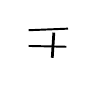
\begin{tikzpicture}[baseline=-.1cm,x=1cm,y=1cm]\draw[line width=.7pt] (0,.18)--(.5,.2);\draw[line width=.7pt] (0,-.02)--(.48,-.03);\draw[line width=1pt] (.32,.15)--(.3,-.17);\end{tikzpicture}}}}\operatorname{Lien}(\underline{G}(\underline{F}_p))$:
\[
0\handwritten{\longrightarrow}H\handwritten{\longrightarrow}G\handwritten{\longrightarrow}G'\handwritten{\mathrel{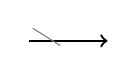
\begin{tikzpicture}[baseline=0cm,x=1cm,y=1cm]\draw[->,thick] (0,0)--(1,0);\draw[gray,thin] (.05,.16)--(.4,-.06);\end{tikzpicture}}}0\ ,
\]
où $H$ est le groupe de t.m. dont le groupe des caractères est le
